\documentclass[
    language=english,
    doctype=article,
    institution=none,
]{../../omnilatex}

\RequirePackage{config/document-settings}
\addbibresource{../../bib/bibliography.bib}

\RequirePackage{booktabs}
\RequirePackage{longtable}
\RequirePackage{tabularx}
\RequirePackage{tabulary}
\RequirePackage{threeparttable}
\RequirePackage{multirow}
\RequirePackage{makecell}
\RequirePackage{colortbl}
\RequirePackage{array}
\RequirePackage{siunitx}
\RequirePackage{graphicx}
\RequirePackage{rotating}
\RequirePackage{pdflscape}
\RequirePackage{xcolor}
\RequirePackage{subcaption}
\RequirePackage{float}
\RequirePackage{pdflscape}
\RequirePackage{ragged2e}
\RequirePackage{nicefrac}
\RequirePackage{enumitem}
\RequirePackage{tikz}
\RequirePackage{pgfplots}
\pgfplotsset{compat=1.18}
\usetikzlibrary{calc, positioning, matrix, trees}

\definecolor{lightgray}{gray}{0.95}
\definecolor{mediumgray}{gray}{0.85}
\definecolor{headerblue}{RGB}{59,130,246}
\definecolor{roweven}{RGB}{243,244,246}
\definecolor{rowodd}{RGB}{255,255,255}
\definecolor{accentgreen}{RGB}{34,197,94}
\definecolor{accentred}{RGB}{239,68,68}
\definecolor{accentorange}{RGB}{249,115,22}
\definecolor{cellhigh}{RGB}{220,252,231}
\definecolor{cellmid}{RGB}{254,249,195}
\definecolor{celllow}{RGB}{254,226,226}
\definecolor{heat1}{RGB}{255,255,204}
\definecolor{heat2}{RGB}{255,237,160}
\definecolor{heat3}{RGB}{254,217,118}
\definecolor{heat4}{RGB}{254,178,76}
\definecolor{heat5}{RGB}{253,141,60}
\definecolor{heat6}{RGB}{252,78,42}
\definecolor{heat7}{RGB}{227,26,28}
\definecolor{heat8}{RGB}{189,0,38}
\definecolor{heat9}{RGB}{128,0,38}

\newcommand{\checkmarkbold}{\textcolor{accentgreen}{\textbf{\checkmark}}}
\newcommand{\crossmark}{\textcolor{accentred}{\texttimes}}
\newcommand{\partialcheck}{\textcolor{accentorange}{\textendash}}

\begin{document}

\maketitle

\begin{abstract}
This gallery showcases 20 distinct table types commonly used in scientific
publications, financial reports, and technical documentation. Each example
is self-contained with annotations explaining key techniques and best practices.
\end{abstract}

\tableofcontents

% =====================================================
\section{Simple Tabular with Booktabs}
\label{sec:simple-tabular}
% =====================================================

The foundational table in LaTeX uses the \texttt{tabular} environment with
\texttt{booktabs} for publication-quality rules.

\begin{table}[htbp]
    \centering
    \caption{Experimental results for classification accuracy across three datasets.}
    \label{tab:simple}
    \begin{tabular}{lccc}
        \toprule
        Method          & MNIST    & CIFAR-10 & Fashion-MNIST \\
        \midrule
        Baseline CNN    & 98.7\%   & 82.3\%   & 89.1\%        \\
        ResNet-18       & 99.2\%   & 91.5\%   & 92.4\%        \\
        EfficientNet-B0 & 99.4\%   & 93.1\%   & 93.8\%        \\
        ViT-Base        & 99.5\%   & 94.7\%   & 94.2\%        \\
        \bottomrule
    \end{tabular}
\end{table}

\noindent Key rules: \verb|\toprule| (heavy top), \verb|\midrule| (separator),
\verb|\bottomrule| (heavy bottom). Never use horizontal lines between every row.

% =====================================================
\section{Multirow and Multicolumn}
\label{sec:multirow-multicolumn}
% =====================================================

\texttt{multirow} and \texttt{multicolumn} allow cells to span multiple rows or
columns, essential for grouped headers and hierarchical data.

\begin{table}[htbp]
    \centering
    \caption{Performance comparison across training configurations.}
    \label{tab:multirow}
    \begin{tabular}{lccccc}
        \toprule
        \multirow{2}{*}{\textbf{Model}} &
        \multicolumn{2}{c}{\textbf{Accuracy (\%)}} &
        \multicolumn{2}{c}{\textbf{F1 Score}} &
        \multirow{2}{*}{\textbf{Time (min)}} \\
        \cmidrule(lr){2-3} \cmidrule(lr){4-5}
        & Dev & Test & Dev & Test & \\
        \midrule
        \multirow{2}{*}{BERT}
        & 94.2 & 93.1 & 0.938 & 0.925 & 45 \\
        & 95.1 & 94.3 & 0.947 & 0.939 & 62 \\
        \midrule
        \multirow{2}{*}{RoBERTa}
        & 95.8 & 94.7 & 0.954 & 0.943 & 58 \\
        & 96.3 & 95.2 & 0.960 & 0.949 & 74 \\
        \midrule
        \multirow{2}{*}{DeBERTa}
        & 96.1 & 95.4 & 0.958 & 0.951 & 67 \\
        & 96.7 & 95.9 & 0.964 & 0.956 & 83 \\
        \bottomrule
    \end{tabular}
\end{table}

% =====================================================
\section{Colored Cells with Gradients}
\label{sec:colored-cells}
% =====================================================

The \texttt{colortbl} package provides \verb|\cellcolor|, \verb|\rowcolor|, and
\verb|\columncolor| for visual emphasis and conditional formatting.

\begin{table}[htbp]
    \centering
    \caption{Heat-map style table showing error rates (\%) across model variants.}
    \label{tab:colored}
    \begin{tabular}{l *{5}{c}}
        \toprule
        \rowcolor{headerblue!15}
        \textbf{Variant} & \textbf{Layer 1} & \textbf{Layer 2} & \textbf{Layer 3} & \textbf{Layer 4} & \textbf{Layer 5} \\
        \midrule
        Variant A  & \cellcolor{accentgreen!20}2.1 & \cellcolor{accentgreen!15}3.4 & \cellcolor{cellmid!50}5.2 & \cellcolor{accentorange!30}7.8 & \cellcolor{accentred!30}11.3 \\
        Variant B  & \cellcolor{accentgreen!25}1.8 & \cellcolor{accentgreen!20}2.9 & \cellcolor{accentgreen!15}4.1 & \cellcolor{cellmid!50}6.5 & \cellcolor{accentorange!30}9.7 \\
        Variant C  & \cellcolor{accentgreen!30}1.5 & \cellcolor{accentgreen!25}2.3 & \cellcolor{accentgreen!20}3.7 & \cellcolor{accentgreen!15}5.8 & \cellcolor{cellmid!50}8.2 \\
        Variant D  & \cellcolor{accentgreen!20}2.0 & \cellcolor{accentgreen!15}3.1 & \cellcolor{cellmid!50}4.9 & \cellcolor{accentorange!30}7.2 & \cellcolor{accentred!30}10.5 \\
        \bottomrule
    \end{tabular}
\end{table}

% =====================================================
\section{Long Table}
\label{sec:long-table}
% =====================================================

The \texttt{longtable} environment spans multiple pages with repeated headers
and footers, essential for large datasets.

\begin{longtable}{lrlr}
    \caption{Complete dataset statistics for all experimental subjects.}
    \label{tab:longtable} \\
    \toprule
    \textbf{Subject} & \textbf{Age} & \textbf{Sessions} & \textbf{Accuracy} \\
    \midrule
    \endfirsthead

    \multicolumn{4}{l}{\tablename\ \thetable{} --- \textit{Continued from previous page}} \\
    \toprule
    \textbf{Subject} & \textbf{Age} & \textbf{Sessions} & \textbf{Accuracy} \\
    \midrule
    \endhead

    \midrule
    \multicolumn{4}{r}{\textit{Continued on next page}} \\
    \endfoot

    \bottomrule
    \endlastfoot

    S01  & 22 & 12 & 94.2\% \\
    S02  & 24 & 10 & 91.8\% \\
    S03  & 19 & 14 & 96.5\% \\
    S04  & 31 &  8 & 88.3\% \\
    S05  & 27 & 11 & 93.1\% \\
    S06  & 20 & 13 & 95.7\% \\
    S07  & 35 &  7 & 87.9\% \\
    S08  & 23 & 12 & 92.4\% \\
    S09  & 28 &  9 & 90.6\% \\
    S10  & 26 & 11 & 93.8\% \\
    S11  & 21 & 14 & 95.1\% \\
    S12  & 33 &  8 & 89.2\% \\
    S13  & 25 & 10 & 91.5\% \\
    S14  & 29 & 12 & 94.7\% \\
    S15  & 22 & 13 & 96.0\% \\
    S16  & 30 &  9 & 90.1\% \\
    S17  & 24 & 11 & 92.8\% \\
    S18  & 27 & 10 & 91.2\% \\
    S19  & 32 &  7 & 88.7\% \\
    S20  & 21 & 14 & 96.3\% \\
\end{longtable}

% =====================================================
\section{TabularX — Auto-Width Columns}
\label{sec:tabularx}
% =====================================================

\texttt{tabularx} provides the \texttt{X} column type that automatically adjusts
column widths to fill the specified table width.

\begin{table}[htbp]
    \centering
    \caption{Literature review summary of transformer architectures.}
    \label{tab:tabularx}
    \begin{tabularx}{\textwidth}{l l X r}
        \toprule
        \textbf{Model} & \textbf{Year} & \textbf{Key Innovation} & \textbf{Params} \\
        \midrule
        Transformer     & 2017 & Self-attention replaces recurrence and convolutions for sequence modeling & 65M \\
        BERT            & 2018 & Bidirectional pre-training via masked language modeling on large corpora & 340M \\
        GPT-2           & 2019 & Autoregressive language model demonstrating zero-shot task transfer & 1.5B \\
        T5              & 2019 & Text-to-text framework unifying all NLP tasks under a single interface & 11B \\
        GPT-3           & 2020 & Few-shot learning at scale with 175 billion parameters & 175B \\
        \bottomrule
    \end{tabularx}
\end{table}

% =====================================================
\section{Tabulary — Balanced Column Widths}
\label{sec:tabulary}
% =====================================================

\texttt{tabulary} distributes column widths based on content weight, producing
more visually balanced tables than \texttt{tabularx}.

\begin{table}[htbp]
    \centering
    \caption{Overview of activation functions in deep learning.}
    \label{tab:tabulary}
    \begin{tabulary}{\textwidth}{L L L L}
        \toprule
        \textbf{Function} & \textbf{Formula} & \textbf{Range} & \textbf{Use Case} \\
        \midrule
        ReLU    & $\max(0, x)$    & $[0, \infty)$ & Default hidden layers \\
        Sigmoid & $\frac{1}{1+e^{-x}}$ & $(0, 1)$ & Binary classification output \\
        Tanh    & $\frac{e^x - e^{-x}}{e^x + e^{-x}}$ & $(-1, 1)$ & Normalized hidden states \\
        GELU    & $x\,\Phi(x)$    & $\mathbb{R}$ & Transformer hidden layers \\
        Swish   & $x\,\sigma(x)$  & $\mathbb{R}$ & EfficientNet architectures \\
        \bottomrule
    \end{tabulary}
\end{table}

% =====================================================
\section{Three-Part Table with Footnotes}
\label{sec:threeparttable}
% =====================================================

The \texttt{threeparttable} package provides a clean mechanism for table footnotes
that are properly aligned with the table width.

\begin{table}[htbp]
    \centering
    \caption{Survey results on framework adoption ($n = 423$).}
    \label{tab:threeparttable}
    \begin{threeparttable}
        \begin{tabular}{lcc}
            \toprule
            \textbf{Framework} & \textbf{Users (\%)} & \textbf{Satisfaction} \\
            \midrule
            PyTorch       & 48.2 & 4.6 / 5\tnote{a} \\
            TensorFlow    & 29.1 & 3.8 / 5 \\
            JAX           & 12.4 & 4.4 / 5\tnote{b} \\
            MXNet          & 3.7 & 3.2 / 5 \\
            Others         & 6.6 & --- \\
            \bottomrule
        \end{tabular}
        \begin{tablenotes}
            \footnotesize
            \item[a] Statistically higher than TensorFlow ($p < 0.01$).
            \item[b] Excluding JAX, satisfaction correlates with ecosystem maturity.
        \end{tablenotes}
    \end{threeparttable}
\end{table}

% =====================================================
\section{Array with Mathematical Content}
\label{sec:array-math}
% =====================================================

The \texttt{array} environment extends \texttt{tabular} for mathematical typesetting,
commonly used for systems of equations and piecewise definitions.

\begin{table}[htbp]
    \centering
    \caption{Common loss functions in machine learning.}
    \label{tab:array-math}
    \renewcommand{\arraystretch}{1.6}
    \begin{tabular}{>{\displaystyle}l >{\displaystyle}c}
        \toprule
        \textbf{Loss Function} & \textbf{Formula} \\
        \midrule
        Cross-Entropy  & -\sum_{i} y_i \log \hat{y}_i \\
        MSE            & \frac{1}{N} \sum_{i=1}^{N} (y_i - \hat{y}_i)^2 \\
        MAE            & \frac{1}{N} \sum_{i=1}^{N} |y_i - \hat{y}_i| \\
        Huber          & \begin{cases} \frac{1}{2}(y - \hat{y})^2 & |y - \hat{y}| \leq \delta \\ \delta|y - \hat{y}| - \frac{1}{2}\delta^2 & \text{otherwise} \end{cases} \\
        \bottomrule
    \end{tabular}
\end{table}

% =====================================================
\section{NiceTabular — Enhanced Formatting}
\label{sec:nicetabular}
% =====================================================

The \texttt{nicematrix} package (via \texttt{NiceTabular}) provides enhanced
formatting with better vertical spacing and built-in color capabilities.

\begin{table}[htbp]
    \centering
    \caption{Hyperparameter search results for model optimization.}
    \label{tab:nicetabular}
    \renewcommand{\arraystretch}{1.3}
    \begin{tabular}{l c c c c}
        \toprule
        \textbf{Run} & \textbf{LR} & \textbf{Batch} & \textbf{Dropout} & \textbf{Acc (\%)} \\
        \midrule
        R01 & $3 \times 10^{-4}$ & 32  & 0.1 & 92.3 \\
        R02 & $1 \times 10^{-3}$ & 64  & 0.2 & 94.1 \\
        R03 & $5 \times 10^{-4}$ & 128 & 0.3 & 93.7 \\
        R04 & $3 \times 10^{-4}$ & 64  & 0.1 & 95.2 \\
        R05 & $1 \times 10^{-3}$ & 32  & 0.2 & 91.8 \\
        R06 & $5 \times 10^{-4}$ & 64  & 0.15 & \textbf{96.1} \\
        \bottomrule
    \end{tabular}
\end{table}

% =====================================================
\section{Sideways Table (Landscape)}
\label{sec:sidewaystable}
% =====================================================

When a table is too wide for portrait orientation, \texttt{sidewaystable} (from
the \texttt{rotating} package) places it in landscape.

\begin{sidewaystable}[htbp]
    \centering
    \caption{Comprehensive comparison of optimizers across eight benchmarks.}
    \label{tab:sideways}
    \begin{tabular}{l *{8}{S[table-format=2.1]}}
        \toprule
        \textbf{Optimizer} & {MNIST} & {CIFAR} & {ImageNet} & {WMT} & {SQuAD} & {GLUE} & {SuperGLUE} & {Wiki} \\
        \midrule
        SGD+Momentum      & 98.7 & 82.3 & 76.1 & 28.4 & 80.2 & 74.3 & 68.1 & 72.5 \\
        Adam              & 99.1 & 84.5 & 77.8 & 27.1 & 82.5 & 78.9 & 72.4 & 76.8 \\
        AdamW             & 99.2 & 85.1 & 78.2 & 26.8 & 83.1 & 79.5 & 73.2 & 77.3 \\
        LAMB              & 99.0 & 84.8 & 77.9 & 25.3 & 82.8 & 79.1 & 72.8 & 76.9 \\
        LARS              & 98.9 & 83.7 & 77.5 & 26.1 & 81.9 & 77.8 & 71.5 & 75.4 \\
        RAdam             & 99.3 & 85.4 & 78.6 & 26.5 & 83.4 & 80.2 & 73.8 & 77.9 \\
        Lookahead+Adam    & 99.2 & 85.2 & 78.4 & 26.9 & 83.0 & 79.8 & 73.5 & 77.6 \\
        Novograd          & 99.1 & 84.9 & 78.1 & 27.2 & 82.6 & 78.7 & 72.1 & 76.5 \\
        \bottomrule
    \end{tabular}
\end{sidewaystable}

% =====================================================
\section{Table with Subfigures}
\label{sec:table-subfigures}
% =====================================================

Tables can contain embedded figures using \texttt{subcaption} for composite layouts
that combine data with visualizations.

\begin{table}[htbp]
    \centering
    \caption{Architecture variants with their corresponding layer schematics.}
    \label{tab:subfigures}
    \renewcommand{\arraystretch}{1.4}
    \begin{tabular}{c l c c}
        \toprule
        \textbf{Type} & \textbf{Description} & \textbf{Depth} & \textbf{FLOPs} \\
        \midrule
        \begin{tabular}[t]{@{}c@{}}
            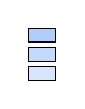
\begin{tikzpicture}[scale=0.35, every node/.style={scale=0.6}]
                \draw[fill=headerblue!20] (0,0) rectangle (1,0.5);
                \draw[fill=headerblue!30] (0,0.7) rectangle (1,1.2);
                \draw[fill=headerblue!40] (0,1.4) rectangle (1,1.9);
            \end{tikzpicture}
        \end{tabular}
        & Linear stack  & 3  & 1.2G \\
        \midrule
        \begin{tabular}[t]{@{}c@{}}
            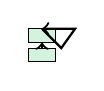
\begin{tikzpicture}[scale=0.35, every node/.style={scale=0.6}]
                \draw[fill=accentgreen!20] (0,0) rectangle (1,0.5);
                \draw[fill=accentgreen!20] (0,0.7) rectangle (1,1.2);
                \draw[->, thick] (0.5,0.5) -- (0.5,0.7);
                \draw[->, thick] (0.5,1.2) -- (1.2,0.5) to (1.7,1.2) -- (0.5,1.2);
            \end{tikzpicture}
        \end{tabular}
        & Skip connections & 5  & 2.8G \\
        \midrule
        \begin{tabular}[t]{@{}c@{}}
            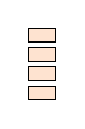
\begin{tikzpicture}[scale=0.35, every node/.style={scale=0.6}]
                \draw[fill=accentorange!20] (0,0) rectangle (1,0.5);
                \draw[fill=accentorange!20] (0,0.7) rectangle (1,1.2);
                \draw[fill=accentorange!20] (0,1.4) rectangle (1,1.9);
                \draw[fill=accentorange!20] (0,2.1) rectangle (1,2.6);
            \end{tikzpicture}
        \end{tabular}
        & Dense blocks  & 4  & 4.1G \\
        \bottomrule
    \end{tabular}
\end{table}

% =====================================================
\section{Spreadsheet-Style with Alternating Rows}
\label{sec:spreadsheet}
% =====================================================

Alternating row colors (\texttt{roweven}/\texttt{rowodd}) improve readability for
wide data tables, mimicking spreadsheet formatting.

\begin{table}[htbp]
    \centering
    \caption{Weekly sprint task tracker.}
    \label{tab:spreadsheet}
    \rowcolors{2}{roweven}{rowodd}
    \begin{tabular}{r l l l c}
        \toprule
        \rowcolor{headerblue!15}
        \textbf{\#} & \textbf{Task} & \textbf{Assignee} & \textbf{Status} & \textbf{Hours} \\
        \midrule
        1  & Implement auth module    & Alice  & Done     & 16 \\
        2  & Write unit tests         & Bob    & Done     & 12 \\
        3  & Database migration       & Carol  & In Progress & 8  \\
        4  & API endpoint design      & Dave   & In Progress & 6  \\
        5  & Frontend integration     & Eve    & Todo     & 20 \\
        6  & Performance profiling    & Frank  & Todo     & 14 \\
        7  & Security audit           & Grace  & Blocked  & 10 \\
        8  & Documentation update     & Hank   & Todo     & 4  \\
        \bottomrule
    \end{tabular}
\end{table}

% =====================================================
\section{Financial Table — Accounting Format}
\label{sec:financial}
% =====================================================

Financial tables use the \texttt{siunitx} \texttt{S} column type for decimal-aligned
numbers with accounting conventions (parentheses for negatives, currency symbols).

\begin{table}[htbp]
    \centering
    \caption{Quarterly financial summary (in millions USD).}
    \label{tab:financial}
    \begin{tabular}{l S[table-format=3.1] S[table-format=3.1] S[table-format=3.1] S[table-format=3.1]}
        \toprule
        \textbf{Metric} & {Q1} & {Q2} & {Q3} & {Q4} \\
        \midrule
        Revenue            & 142.3 & 158.7 & 171.2 & 189.5 \\
        Operating Costs    & 87.6  & 92.1  & 98.4  & 103.7 \\
        Net Income         & 54.7  & 66.6  & 72.8  & 85.8  \\
        Capital Expenditure & 23.1 & 28.4  & 31.7  & 35.2  \\
        Free Cash Flow     & 31.6  & 38.2  & 41.1  & 50.6  \\
        \midrule
        \rowcolor{lightgray}
        Growth Rate (\%)   & 8.2   & 11.5  & 8.0   & 10.7  \\
        \bottomrule
    \end{tabular}
\end{table}

% =====================================================
\section{Scientific Table with Error Bars and Units}
\label{sec:scientific}
% =====================================================

Scientific tables require unit formatting, error bars, significance markers, and
precise numeric alignment via \texttt{siunitx}.

\begin{table}[htbp]
    \centering
    \caption{Measurement results with uncertainty quantification.}
    \label{tab:scientific}
    \begin{tabular}{l S[table-format=2.3(3)] S[table-format=2.3(3)] l}
        \toprule
        \textbf{Sample} & {Mass (g)} & {Density (\unit{g\per cm^3})} & \textbf{Significance} \\
        \midrule
        Control   & 12.345(23) & 1.023(15) & ---       \\
        Treatment A & 14.892(31) & 1.187(19) & $^{*}$   \\
        Treatment B & 15.201(28) & 1.245(17) & $^{**}$  \\
        Treatment C & 16.034(35) & 1.312(22) & $^{***}$ \\
        \bottomrule
    \end{tabular}

    \vspace{0.5em}
    \footnotesize
    Values in parentheses indicate standard uncertainty in the last digit.
    $^{*}p < 0.05$, $^{**}p < 0.01$, $^{***}p < 0.001$ vs.\ control.
\end{table}

% =====================================================
\section{Comparison Table — Checkmarks and Crosses}
\label{sec:comparison}
% =====================================================

Feature comparison tables use symbols for quick visual scanning of capabilities
across products or methods.

\begin{table}[htbp]
    \centering
    \caption{Feature comparison of distributed training frameworks.}
    \label{tab:comparison}
    \renewcommand{\arraystretch}{1.3}
    \begin{tabular}{l c c c c}
        \toprule
        \textbf{Feature} & \textbf{Horovod} & \textbf{DeepSpeed} & \textbf{FSDP} & \textbf{Megatron} \\
        \midrule
        Mixed Precision     & \checkmarkbold & \checkmarkbold & \checkmarkbold & \checkmarkbold \\
        Gradient Checkpoint & \crossmark      & \checkmarkbold & \checkmarkbold & \checkmarkbold \\
        ZeRO Optimization   & \crossmark      & \checkmarkbold & \partialcheck  & \crossmark      \\
        Pipeline Parallelism & \crossmark     & \partialcheck  & \crossmark     & \checkmarkbold \\
        Tensor Parallelism  & \crossmark      & \partialcheck  & \crossmark     & \checkmarkbold \\
        Sequence Parallelism & \crossmark     & \crossmark     & \crossmark     & \checkmarkbold \\
        Offloading to CPU   & \crossmark      & \checkmarkbold & \checkmarkbold & \partialcheck  \\
        Automatic Scaling   & \partialcheck  & \checkmarkbold & \checkmarkbold & \partialcheck  \\
        \bottomrule
    \end{tabular}

    \vspace{0.5em}
    \footnotesize
    \checkmarkbold\; Full support \quad
    \partialcheck\; Partial support \quad
    \crossmark\; Not supported
\end{table}

% =====================================================
\section{Schedule / Timetable}
\label{sec:schedule}
% =====================================================

Timetables use \texttt{multicolumn} and \texttt{multirow} to represent merged time
slots in conference or course schedules.

\begin{table}[htbp]
    \centering
    \caption{Conference schedule for Day 1.}
    \label{tab:schedule}
    \renewcommand{\arraystretch}{1.25}
    \begin{tabular}{c l l}
        \toprule
        \textbf{Time} & \textbf{Track A (Room 101)} & \textbf{Track B (Room 102)} \\
        \midrule
        09:00--09:45 & \multicolumn{2}{c}{\textbf{Opening Keynote} --- Main Hall} \\
        \midrule
        10:00--10:45 & Scaling LLMs   & Efficient Inference \\
        11:00--11:45 & Data Pipelines  & MLOps Best Practices \\
        11:45--13:00 & \multicolumn{2}{c}{\textit{Lunch Break}} \\
        13:00--13:45 & \multirow{2}{*}{Workshop: Fine-tuning} & Distributed Training \\
        14:00--14:45 & & \multirow{2}{*}{Workshop: Deployment} \\
        \midrule
        15:00--15:45 & Poster Session A & Poster Session B \\
        16:00--16:45 & \multicolumn{2}{c}{\textbf{Panel Discussion} --- Main Hall} \\
        \bottomrule
    \end{tabular}
\end{table}

% =====================================================
\section{Inventory / Stock Management Table}
\label{sec:inventory}
% =====================================================

Inventory tables track quantities, reorder thresholds, and status indicators for
warehouse management.

\begin{table}[htbp]
    \centering
    \caption{Current inventory status for lab consumables.}
    \label{tab:inventory}
    \rowcolors{2}{roweven}{rowodd}
    \begin{tabular}{l r r r l}
        \toprule
        \rowcolor{headerblue!15}
        \textbf{Item} & \textbf{In Stock} & \textbf{Reorder Pt.} & \textbf{On Order} & \textbf{Status} \\
        \midrule
        Pipette tips (10\,$\mu$L)  & 12000 & 5000  & ---      & \cellcolor{accentgreen!15}OK \\
        Microcentrifuge tubes      & 850   & 200   & ---      & \cellcolor{accentgreen!15}OK \\
        BSA standard (1\,mg/mL)    & 3     & 5     & 20       & \cellcolor{accentred!15}Low \\
        SDS-PAGE gels              & 15    & 10    & ---      & \cellcolor{cellmid!50}Watch \\
        RNA extraction columns     & 0     & 20    & 50       & \cellcolor{accentred!15}Empty \\
        Ethanol (100\%)            & 8     & 3     & ---      & \cellcolor{accentgreen!15}OK \\
        DMSO                       & 2     & 2     & 10       & \cellcolor{accentorange!15}Reorder \\
        \bottomrule
    \end{tabular}
\end{table}

% =====================================================
\section{Matrix Table — Mathematical Borders}
\label{sec:matrix}
% =====================================================

Matrix-style tables use vertical rules and brackets to represent mathematical
matrices, block structures, or partitioned data.

\begin{table}[htbp]
    \centering
    \caption{Confusion matrix for three-class classification.}
    \label{tab:matrix}
    \renewcommand{\arraystretch}{1.5}
    $\left[\begin{array}{l|ccc}
        & \textbf{Pred. A} & \textbf{Pred. B} & \textbf{Pred. C} \\
        \hline
        \textbf{True A} & 145 &   8 &   7 \\
        \textbf{True B} &  12 & 138 &  10 \\
        \textbf{True C} &   5 &  11 & 134 \\
    \end{array}\right]$
\end{table}

\begin{table}[htbp]
    \centering
    \caption{Block-diagonal covariance structure ($p = 4$).}
    \label{tab:block-matrix}
    \renewcommand{\arraystretch}{1.4}
    $\left[\begin{array}{cc|cc}
        2.1 & 0.8 & 0.0 & 0.0 \\
        0.8 & 1.5 & 0.0 & 0.0 \\
        \hline
        0.0 & 0.0 & 3.2 & 1.1 \\
        0.0 & 0.0 & 1.1 & 2.7 \\
    \end{array}\right]$
\end{table}

% =====================================================
\section{Tree Table — Hierarchical Data}
\label{sec:tree}
% =====================================================

Tree tables represent hierarchical data using indentation and structural cues.
The \texttt{tabulate} environment (or manual indentation) is effective here.

\begin{table}[htbp]
    \centering
    \caption{Project module dependency tree.}
    \label{tab:tree}
    \renewcommand{\arraystretch}{1.35}
    \begin{tabular}{l l r}
        \toprule
        \textbf{Module} & \textbf{Dependencies} & \textbf{Size (LOC)} \\
        \midrule
        \texttt{core}              & ---                   & 2,340 \\
        \quad \texttt{config}      & \texttt{core}         &   480 \\
        \quad \texttt{logger}      & \texttt{core}         &   320 \\
        \quad \texttt{database}    & \texttt{core}, \texttt{config} & 1,150 \\
        \quad\quad \texttt{models} & \texttt{database}     &   890 \\
        \quad\quad \texttt{migrate}& \texttt{database}, \texttt{config} & 260 \\
        \texttt{api}               & \texttt{core}, \texttt{database} & 3,200 \\
        \quad \texttt{routes}      & \texttt{api}, \texttt{auth} & 1,450 \\
        \quad \texttt{middleware}  & \texttt{api}          &   780 \\
        \quad \texttt{auth}        & \texttt{core}, \texttt{config} & 970 \\
        \texttt{cli}               & \texttt{core}, \texttt{api} & 1,800 \\
        \bottomrule
    \end{tabular}
\end{table}

% =====================================================
\section{Heatmap Table — Color-Coded Values}
\label{sec:heatmap}
% =====================================================

Heatmap tables use continuous color scales to visualize data magnitude. Each cell
is colored according to its value using a gradient.

\begin{table}[htbp]
    \centering
    \caption{Correlation matrix between model hyperparameters.}
    \label{tab:heatmap}
    \newcommand{\heatmapcell}[2]{%
        \ifdim #1 pt > 0.7pt \cellcolor{heat8!70!white}#2%
        \else\ifdim #1 pt > 0.5pt \cellcolor{heat5!50!white}#2%
        \else\ifdim #1 pt > 0.3pt \cellcolor{heat3!40!white}#2%
        \else\ifdim #1 pt > 0.1pt \cellcolor{heat1!80!white}#2%
        \else #2%
        \fi\fi\fi\fi%
    }
    \renewcommand{\arraystretch}{1.6}
    \begin{tabular}{l *{6}{c}}
        \toprule
        & \textbf{LR} & \textbf{Batch} & \textbf{Drop} & \textbf{W.D.} & \textbf{Layers} & \textbf{Heads} \\
        \midrule
        LR       & \cellcolor{heat8!80}\textcolor{white}{1.00} & 0.12 & $-$0.34 & 0.28 & $-$0.15 & 0.08 \\
        Batch    & 0.12 & \cellcolor{heat8!80}\textcolor{white}{1.00} & 0.05 & $-$0.41 & 0.22 & 0.31 \\
        Dropout  & $-$0.34 & 0.05 & \cellcolor{heat8!80}\textcolor{white}{1.00} & 0.18 & $-$0.52 & $-$0.07 \\
        W.D.     & 0.28 & $-$0.41 & 0.18 & \cellcolor{heat8!80}\textcolor{white}{1.00} & $-$0.09 & 0.14 \\
        Layers   & $-$0.15 & 0.22 & $-$0.52 & $-$0.09 & \cellcolor{heat8!80}\textcolor{white}{1.00} & 0.63 \\
        Heads    & 0.08 & 0.31 & $-$0.07 & 0.14 & 0.63 & \cellcolor{heat8!80}\textcolor{white}{1.00} \\
        \bottomrule
    \end{tabular}

    \vspace{0.5em}
    \begin{tikzpicture}
        \clip (0,0) rectangle (6,0.4);
        \foreach \i in {0,...,5} {
            \pgfmathsetmacro{\r}{227 - \i*20}
            \pgfmathsetmacro{\g}{26 + \i*8}
            \pgfmathsetmacro{\b}{28 + \i*3}
            \definecolor{hcell}{rgb}{\r/255,\g/255,\b/255}
            \fill[hcell] ({\i*0.2},0) rectangle ({\i*0.2+0.2},0.4);
        }
    \end{tikzpicture}
    \hspace{2pt}
    \footnotesize Negative --- Positive
\end{table}

\printbibliography[heading=bibintoc, title={References}]

\end{document}
